\chapter{Introduction and Theory Overview}

\section{Introduction}
This thesis presents the analysis details and the results of the search for heavy resonances decaying into a $Z$ boson and a Higgs boson (h) at the center-of-mass energy of 8 TeV, using 19.7 fb$^{-1}$ p-p collision data. In turn, the $Z$ boson is identified through its leptonic decays (leptons often refer to $e$ and $\mu$ only in experiments. $l = e, \mu$). The Higgs boson h is expected to hadronically decay into a pair of b-quarks. The investigated final states consist of two charged leptons which are identified in the detector and limit the presence of the background, and two b-quarks from the hadronic Higgs decay which collects the largest possible fraction of Higgs events.
\newline This thesis is organised as follows. In the latter part of this chapter, the model that predicts heavy resonances is introduced, including the expected cross section and the specification of model parameters. In chapter 2, the LHC and the CMS experiment are described, including the information of each sub-detector and the trigger system of the CMS. The details of the analysis are shown in chapter 3. This chapter reveals the way to reconstruct physical objects in CMS. By adding some proper kinematic selections on those physics objects, the interested events in data collected by the CMS detector can be selected. Moreover, this chapter shows the comparison between data and simulation. In the last chapter, the results of the search and the conclusion are presented.

\section{Theory Overview}
Although the Higgs boson discovered by the ATLAS and CMS collaborations\cite{atlas-higgs-1,cms-higgs-1,cms-higgs-2} imposes strong constraints on theories beyond the Standard Model(SM), the extreme fine tuning in quantum corrections required to have a light fundamental Higgs boson with mass close to 125 GeV\cite{cms-higgs-3,atlas-higgs-2,atlas-higgs-3,atlas-cms-higgs} suggests that the Standard Model may be incomplete, and not valid beyond a scale of a few TeV. Various dynamical electroweak symmetry breaking scenarios which attempt to solve this naturalness problem, such as Minimal Walking Technicolor\cite{technicolor}, Little Higgs\cite{little-higgs-1,little-higgs-2,little-higgs-3}, or composite Higgs models\cite{compositehiggs-1,compositehiggs-2,compositehiggs-3} predict the existence of new resonances decaying to a vector boson plus a Higgs boson.

\subsection{Heavy Vector Triplet Model}
Resonance searches are typically not sensitive to all the details and the free parameters of the underlying model, but only to those parameters or combinations of parameters that control the mass of the resonance and the interactions involved in its production and decay. Therefore, one can employ a simplified description of the resonance defined by a phenomenological Lagrangian where only the relevant couplings and mass parameters are retained. This model-independent strategy applies a Heavy Vector Triplet (HVT)\cite{HVT} to the Standard Model group and reproduces a large class of explicit models. In Eq.~(\ref{eq:phen-Lag}), the mathematical form of the simplified Lagrangian is defined, where $V_{\nu}^{a}$ , $a$ = 1,2,3, is a real vector with vanishing hypercharge in the adjoint representation of $SU(2)_{L}$, it decscribes one charged and one neutral heavy spin-1 particle with charge eigenstate fields, and $D_{[\mu}V_{\nu]}^{a}$ represents the covariant derivative.

\begin{align} 
  \label{eq:phen-Lag}
  \mathcal{L}_{\mathcal{V}} =& -\frac{1}{4}D_{[\mu}V_{\nu]}^{a}D^{[\mu}V^{\nu] a}+\frac{{m_{V}^{2}}}{2}V_{\mu}^{a}V^{\mu a}\nonumber\\&+ig_{V}c_{H}V_{\mu}^{a}H^{\dagger}{\tau}^{a}{\overset{\text{\scriptsize$\leftrightarrow$}}{D}}^{\mu}H+\frac{g^{2}}{g_{V}}c_{F}V_{\mu}^{a}\sum_{f}\bar{f}_{L}{\gamma}^{\mu}{\tau}^{a}f_{L}\nonumber\\&+\frac{g_{V}}{2}c_{VVV}\epsilon_{abc}V_{\mu}^{a}V_{\nu}^{b}D^{[\mu}V^{\nu] c}+\textup{quadrilinear terms}
\end{align}

\begin{align}
  V_{\mu}^{\pm}=\frac{V_{\mu}^{1}\mp iV_{\mu}^{2}}{\sqrt{2}}\textup{ , }V_{\mu}^{0}=V_{\mu}^{3}
\end{align}
\begin{align}
  D_{[\mu}V_{\nu]}^{a} = D_{\mu}V_{\nu}^{a}-D_{\nu}V_{\mu}^{a}\textup{ , }D_{\mu}V_{\nu}^{a}=\partial_{\mu}V_{\nu}^{a}+g\epsilon^{abc}W_{\mu}^{b}V_{\nu}^{c}
\end{align}
\newline In these models, new heavy vector bosons ($V^{\pm}, V^{0}$) that couple to the Higgs and SM gauge bosons with the parameters $c_{H}$ and $g_{V}$ and to the fermions via the combination $(g^{2}/g_{V})c_{F}$ . The parameter $g_{V}$ represents the strength of the new vector boson interaction, while $c_{H}$ and $c_{F}$ represent the couplings to the Higgs and the fermions respectively, and are expected to be of the order of unity in most models. 


\subsection{Basic Phenomenology}
\subsection*{Masses and Mixings}
After electro-weak symmetry breaking (EWSB), the only massless state is photon, which can be identified as the gauge field associated with the unbroken $U(1)_{em}$. The two other neutral mass eigenstates are the SM $Z$ boson and one heavy vector of mass $M_{0}$ which are obtained by diagonalizing the mass matrix of the ($Z,V^{0}$) system by a rotation with angle $\theta_{N}$
\begin{align}
  \begin{pmatrix}
    Z\\
    V^{0}
  \end{pmatrix}
  \rightarrow
  \begin{pmatrix}
    \cos{\theta_{N}} & \sin{\theta_{N}}\\
    -\sin{\theta_{N}}& \cos{\theta_{N}}
  \end{pmatrix}
  \begin{pmatrix}
    Z\\
    V^{0}
  \end{pmatrix}
  .
\end{align}
The mass matrix is
\begin{align}
  \label{eq:MassMatrixN}
  \mathcal{M}_{N}^{2}=
  \begin{pmatrix}
    \hat{m}_{Z}^{2} & c_{H}\xi \hat{m}_{Z} \hat{m}_{V}\\
    c_{H}\xi \hat{m}_{Z} \hat{m}_{V} & \hat{m}_{V}^{2}
  \end{pmatrix}
  \textup{ , where}
  \begin{cases}
    \hat{m}_{Z}=\frac{e\hat{\upsilon}}{2\sin{\theta_{W}}\cos{\theta_{W}}}\\
    \hat{m}_{V}^{2}=m_{V}^{2}+g_{V}^{2}c_{VVHH}\hat{\upsilon}^{2}\\
    \xi=\frac{g_{V}\hat{\upsilon}}{2\hat{m}_{V}}
  \end{cases}
  .
\end{align}
In the above equations $\hat{\upsilon}$ denotes the Vacuum Expetation Value (VEV) defined by $\big \langle H^{\dagger}H\big \rangle=\hat{\upsilon}^{2}/2$, and one should know the masses $\hat{m}_{Z}$ and $\hat{m}_{V}$ do not coincide with the physical $Z$ boson and the masses of the new resonances of this model, although they do in the approximations later. The mass eigenvalues and the rotation angles are easily obtained by inverting the relations
\begin{align}
  \label{eq:detMN}
  &Tr[\mathcal{M}_{N}^{2}]=\hat{m}_{Z}^{2}+\hat{m}_{V}^{2}=m_{Z}^{2}+M_{0}^{2}\textup{ ,}\nonumber\\
  &Det[\mathcal{M}_{N}^{2}]=\hat{m}_{Z}^{2}\hat{m}_{V}^{2}(1-c_{H}^{2}\xi^{2})=m_{Z}^{2}M_{0}^{2}\textup{ ,}\nonumber\\
  &\tan{2\theta_{N}}=\frac{2c_{H}\xi \hat{m}_{Z} \hat{m}_{V}}{\hat{m}_{V}^{2}-\hat{m}_{Z}^{2}}\textup{ .}
\end{align}
Notice that the tangent can be uniquely inverted because the angle $\theta_{N}$ is in the range $[-\pi/4,\pi/4]$ in the parameter region we will be interested in, where $\hat{m}_{Z}<\hat{m}_{V}$.
\newline The situation is similar in the charged vector where the mass matrix of the ($W^{\pm},V^{\pm}$) system reads
\begin{align}
  \label{eq:MassMatrixC}
  \mathcal{M}_{C}^{2}=
  \begin{pmatrix}
    \hat{m}_{W}^{2} & c_{H}\xi \hat{m}_{W} \hat{m}_{V}\\
    c_{H}\xi \hat{m}_{W} \hat{m}_{V} & \hat{m}_{V}^{2}
  \end{pmatrix}
  \textup{ , where }
  \hat{m}_{W}=\frac{e\hat{\upsilon}}{2\sin{\theta_{W}}}=\cos{\theta_{W}}\hat{m}_{Z}
  \textup{ ,}
\end{align}
and it is diagonalized by
\begin{align}
  \label{eq:detMC}
  &Tr[\mathcal{M}_{C}^{2}]=\hat{m}_{W}^{2}+\hat{m}_{V}^{2}=m_{W}^{2}+M_{\pm}^{2}\textup{ ,}\nonumber\\
  &Det[\mathcal{M}_{C}^{2}]=\hat{m}_{W}^{2}\hat{m}_{V}^{2}(1-c_{H}^{2}\xi^{2})=m_{W}^{2}M_{\pm}^{2}\textup{ ,}\nonumber\\
  &\tan{2\theta_{C}}=\frac{2c_{H}\xi \hat{m}_{W} \hat{m}_{V}}{\hat{m}_{V}^{2}-\hat{m}_{W}^{2}}\textup{ .}
\end{align}
By checking Eq.~(\ref{eq:MassMatrixN}) and Eq.~(\ref{eq:MassMatrixC}), the charged and neutral mass matrices are connected by custodial symmetry, which can be shown in full generality to imply
\begin{align}
  \mathcal{M}_{C}^{2}=
  \begin{pmatrix}
    \cos{\theta_{W}} & 0\\
    0&1
  \end{pmatrix}
  \mathcal{M}_{N}^{2}
  \begin{pmatrix}
    \cos{\theta_{W}} & 0\\
    0&1
  \end{pmatrix}
  \textup{ .}
\end{align}
By taking the determinant of the above equation, or equivalently by comparing the charged and neutral determinants in Eq.~(\ref{eq:detMN}) and Eq.~(\ref{eq:detMC}), we obtain a generalized custodial relation among the physical masses
\begin{align}
  \label{eq:custRelation}
m_{W}^{2}M_{\pm}^{2}=\cos^{2}\theta_{W}m_{Z}^{2}M_{0}^{2}\textup{ .}
\end{align}
From the simple formula above, we can start to identify the physically reasonable region of the parameter space in this model. We aim at describing new vectors with masses at or above the TeV scale, but we also want the SM masses $m_{W,Z} \sim$ 100 GeV to be reproduced. Therefore we require a hierachy in the mass relation of SM $Z$ and $W$ bosons versus the new vectors.
\begin{align}
  \label{eq:hierachyEq}
  \frac{\hat{m}_{W,Z}}{\hat{m}_{V}}\sim \frac{m_{W,Z}}{M_{\pm ,0}}\leq10^{-1}\ll1
\end{align}
In the limit of Eq.~(\ref{eq:hierachyEq}) we obtain simple approximation for $m_{W}$ and $m_{Z}$
\begin{align}
  &m_{Z}^{2}=\hat{m}_{Z}^{2}(1-c_{H}^{2}\xi^{2})(1+\mathcal{O}(\hat{m}_{Z}^{2}/\hat{m}_{V}^{2}))\textup{ ,}\nonumber\\
  &m_{W}^{2}=\hat{m}_{W}^{2}(1-c_{H}^{2}\xi^{2})(1+\mathcal{O}(\hat{m}_{W}^{2}/\hat{m}_{V}^{2}))\textup{ .}
\end{align}
The parameter $\xi$ can be either very small or of order unity. Both cases are realized in explicit models. While $\xi\ll1$ is the most common situation, $\xi\sim1$ only occurs in strongly coupled scenarios at very large $g_{V}$. In these approximations, SM tree-level experimental observation can be reproduced to percent accuracy.
\newline Since $\hat{m}_{W}=\cos\theta_{W}\hat{m}_{Z}$, the $W$-$Z$ mass ratio is thus given by
\begin{align}
  \label{eq:fracWZ}
  \frac{m_{W}^{2}}{m_{Z}^{2}}\simeq \cos^{2}{\theta_{W}}\textup{ .}
\end{align}
Eq.~(\ref{eq:fracWZ}) has one important implication on the masses of the new vectors. When combined with the custodial relation Eq.~(\ref{eq:custRelation}), it tells us that the charged and neutral $V$s are practically degenerate
\begin{align}
  M_{\pm}^{2}=M_{0}^{2}(1+\mathcal{O}(\%))\textup{ ,}
\end{align}
In the following, when working at the leading order in the limit Eq.~(\ref{eq:hierachyEq}), we can ignore the mass splitting and denote the mass of the charged and the neutral states collectively as $M_{V}$. It is easy to check that in that limit $M_{V}=\hat{m}_{V}$.

\subsection*{Decay Widths}
Because of the hierachy in the mass matrices, the mixing angles are naturally small. By looking at Eqs.~(\ref{eq:detMN}), (\ref{eq:detMC}) and (\ref{eq:hierachyEq}) we can estimate
\begin{align}
  \theta_{N,C}\simeq c_{H}\xi \frac{\hat{m}_{W,Z}}{\hat{m}_{V}}\leq10^{-1}\textup{ ,}
\end{align}
and after rotating to the mass basis, the coupling of the neutral and charged resonances to left- and right-handed fermion chiralities can be written in a compact form for each fermion species $F=\{l,q,3\}$.
\begin{align}
\begin{cases}  
  g_{L}^{N}=\frac{g^{2}}{g_{V}}\frac{c_{F}}{2}\cos\theta_{C}+(g_{L}^{Z})_{SM}\sin\theta_{N}\simeq\frac{g^{2}}{g_{V}}\frac{c_{F}}{2}\textup{ ,}\\
  g_{R}^{N}=(g_{R}^{Z})_{SM}\sin\theta_{N}\simeq0
\end{cases}\nonumber\\
\begin{cases}
  g_{L}^{C}=\frac{g^{2}}{g_{V}}\frac{c_{F}}{2}\cos\theta_{C}+(g_{L}^{W})_{SM}\sin\theta_{C}\simeq\frac{g^{2}}{g_{V}}\frac{c_{F}}{2}\textup{ ,}\\
  g_{R}^{C}=0
\end{cases}
\end{align}
In the above equation $(g_{L,R}^{W,Z})_{SM}$ denote the ordinary SM $W$ and $Z$ couplings (with the normalization given by $g_{L}^{W}=g/\sqrt{2}$).\\
\newline Given that the rotation angles are small, the couplings further simplify, as also shown in the equation. We could see that $V$ interact mainly with left-handed chiralities and that all the couplings for each fermion species are controlled by the parameter combination $g^{2}/g_{V}c_{F}$. This gives tight correlations among different channels
\begin{align}
  \label{eq:DRfermion}
  \Gamma_{V_{\pm}\rightarrow f\bar{f}'}\simeq2\Gamma_{V_{0}\rightarrow f\bar{f}'}\simeq N_{C}[f](\frac{g^{2}c_{F}}{g_{V}})^{2}\frac{M_{V}}{48\pi}\textup{ ,}
\end{align}
where $N_{C}[f]$ is the number of colors (3 for the di-quark and 1 for the dilepton decays). The parameters $c_{F}=\{c_{l},c_{q},c_{3}\}$ control the relative BRs to leptons, light quarks and the third family.
\newline In the case of di-boson decay width
\begin{align}
  \label{eq:DRboson}
  &\Gamma_{V_{0}\rightarrow W_{L}^{+}W_{L}^{-}}\simeq\Gamma_{V_{\pm}\rightarrow W_{L}^{\pm}Z_{L}}\simeq\frac{g_{V}^{2}c_{H}^{2}M_{V}}{192\pi}\frac{(1+c_{H}c_{VVV}\xi^{2})^{2}}{(1-c_{H}^{2}\xi^{2})^{2}}=\frac{g_{V}^{2}c_{H}^{2}M_{V}}{192\pi}[1+\mathcal{O}(\xi^{2})]\textup{ ,}\nonumber\\
  &\Gamma_{V_{0}\rightarrow Z_{L}h}\simeq\Gamma_{V_{\pm}\rightarrow W_{L}^{\pm}h}\simeq\frac{g_{V}^{2}c_{H}^{2}M_{V}}{192\pi}\frac{(1-4c_{VVHH}\xi^{2})^{2}}{1-c_{H}^{2}\xi^{2}}=\frac{g_{V}^{2}c_{H}^{2}M_{V}}{192\pi}[1+\mathcal{O}(\xi^{2})]\textup{ .}\nonumber\\
\end{align}
Note that Eq.~(\ref{eq:DRboson}) is derived in the Equivalent Gauge\cite{EquivGauge} because the decay to transverse SM vectors is highly suppressed while to the longitudinal parts grows with the energy of the process, therefore the Unitary Gauge which is used in the original Lagrangian is instead useful. The channels that are not shown in the above equations are either forbidden, like $hh$ and $\gamma\gamma$ decays, or suppressed like the decays to transverse polarizations.
\newline From this section, a very simple picture emerges. At small $\xi$, all the decay widths are fixed with a given resonance mass $M_{V}$ and the couplings $\{g^{2}c_{F}/g_{V}$, $g_{V}c_{H}\}$ which control the BRs in all relevant channels. Paremeters $c_{VVV},\textup{ } c_{VVHH}\textup{ and }c_{VVW}$ are basically irrelevent. Thus, the basic phenomenology of this model is well described by a good approximation.


\newpage
\subsection{Explicit Models}
Now the general picture is clear, we can get exact values of the widths and BRs from explicit models. Consider two benchmark models, A and B, which correspond to two explicit models describing the heavy vectors in Refs.~\cite{modelA} and \cite{compositehiggs-1} respectively. All the $c$ parameters are fixed to specific values in these models and the only free parameters are the resonance mass $M_{V}$ and coupling $g_{V}$. Moreover, model A is inspired by weakly coupled extensions of the SM gauge group while model B is by strongly coupled scenarios of EWSB, $i.e.$ Composite Higgs models, we will consider them in different regions of $g_{V}$, relatively small $g_{V}\leq3$ and relatively large $g_{V}\geq3$.\\
\newline Figure \ref{fig:BRs_AvsB} shows the BRs as functions of the mass in model A and B. As expected from the previous discussion and according to Refs.~\cite{modelA}, model A predicts
\begin{align}
  \label{eq:DeterA}
  &c_{H}=-g^{2}/g_{V}^{2}\textup{ , }c_{F}\simeq 1 \textup{ ,} \nonumber\\
  &|g_{V}c_{H}|\simeq g^{2}c_{F}/g_{V}\simeq g^{2}/g_{V}\textup{ .}
\end{align}
Therefore Eq.~(\ref{eq:DRfermion}) and (\ref{eq:DRboson}) can be determined in the following form for $V_{0}$ in model A ($g_{V}=1$),
\begin{align}
  &\Gamma_{V_{0}\rightarrow f\bar{f}'}\simeq N_{c}[f]\frac{g^{4}M_{V}}{96\pi}\nonumber\\
  &\Gamma_{V_{0}\rightarrow W^{+}W^{-}}\simeq \Gamma_{V_{0}\rightarrow Zh}\simeq \frac{g^{4}M_{V}}{192\pi}\textup{ .}
\end{align}
One can easily check either from the plot or the equation, a factor of two difference comparing the BRs between fermions and bosons. Due to the color factor, leptons and quarks also have a difference by a factor of three. Since the $c_{F}$ term is universal both in A and B. The total width in model A decreases with increasing $g_{V}$ because of the overall suppresion ($g^{2}/g_{V}$) in Eq.~(\ref{eq:DeterA}).\\On the contrary, in model B the $c_{H}$ term is unsuppressed
\begin{align}
  \label{eq:DeterB}
  &c_{H}\simeq c_{F}\simeq 1 \textup{ ,}\nonumber\\
  &g_{V}c_{H}\simeq-g_{V}\textup{ , }g^{2}c_{c_{F}}/g_{g_{V}}\simeq g^{2}/g_{V}\textup{ .}
\end{align}
Thus the determinate $V_{0}$ decay widths for model B ($g_{V}=3$) are
\begin{align}
  &\Gamma_{V_{0}\rightarrow f\bar{f}'}\simeq N_{c}[f]\frac{g^{4}M_{V}}{342\pi}\nonumber\\
  &\Gamma_{V_{0}\rightarrow W^{+}W^{-}}\simeq \Gamma_{V_{0}\rightarrow Zh}\simeq \frac{3M_{V}}{64\pi}\textup{ .}
\end{align}
For model B$_{g_{V}=3}$ the dominant BRs are into di-bosons and the fermionic decays are extremely suppressed. Moreover, the total width increases with increasing $g_{V}$ since it is dominated by the di-boson width which grows with $g_{V}$ as expected from Eq.~({\ref{eq:DeterB}}). This model B is particularly interesting for the present search, since it predicts signal cross sections in order of fb\cite{HVT} \cite{CMS_AN_2015-186}, branching ratios to vector bosons close to unity, and thus being accessible at the LHC. In the latter chapters, the mass eigenstate of the neutral heavy vector boson in model B scenario refers to the $Z'$ particle, which is the search target of this thesis.\\
\begin{figure}[h]
  \begin{center}
    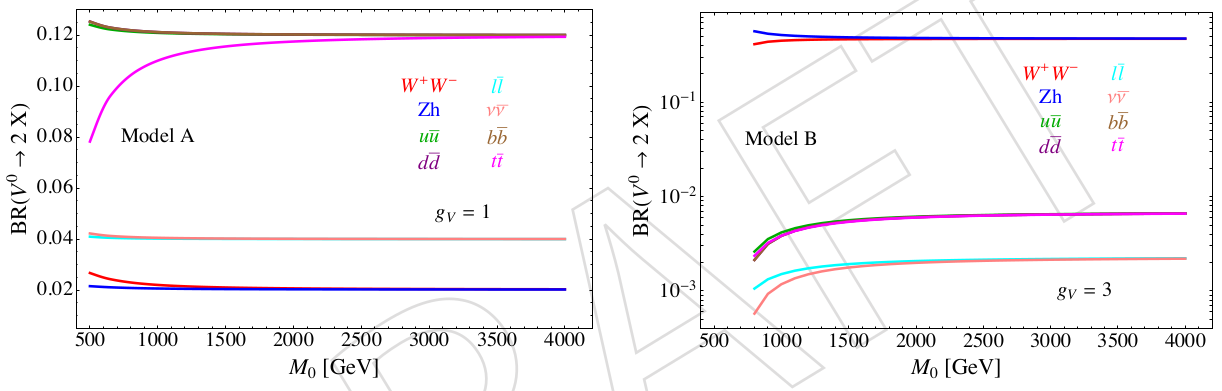
\includegraphics[width=\textwidth]{figure/CH1/BRs_modelAvsB.png}
  \end{center}
  \caption{\label{fig:BRs_AvsB}Branching ratios as a function of the resonance mass for the HVT benchmark model A(left) and model B(right).}
\end{figure}
